\chapter{Regularisation for Interpreting Weights and Loadings}\label{chap:als}
\minitoc

\section{Introduction}\label{sec:introduction}

This chapter is an extension of work that I have previously presented in poster form at the OHBM conference.
I have benefitted from constructive theoretical discussions with John Shawe-Taylor and Janaina Mourao-Miranda, as well as insights into result interpretation from Janaina and Rick Adams.

When applying CCA methods to practical problems, we may be interested in both predicting latent variables associated
with different views (the backward problem \cite{haufe2014interpretation}), as well as understanding the relationship between the views (the forward problem).

This is somewhat similar to the distinction between machine learning and statistical approaches to the CCA problem.
In the former, we are motivated by (out-of-sample) prediction, while in the latter we are interested in inferring the
data generation process.

In practice, we are often interested in both prediction and inference. We would ideally like to have the best
possible prediction of the latent variables, while also being able to interpret the model and understand the
relationship between the views.

Traditional CCA models often exhibit shortcomings when grappling with high-dimensional data, a challenge particularly
acute in the context of brain-behavior studies. They are prone to overfitting, leading to spurious correlations and
poor generalization.

Regularization is a powerful tool for addressing linear models. It can help us avoid overfitting and improve the
interpretability of the results. However structured regularization like the Lasso

This chapter will explore the role of regularization in CCA. We will show that regularization is most helpful when it
allows us to align the model's objective with the characteristics of the underlying signal. We will argue that
regularization can be used to improve both prediction and interpretation.

\section{Background}\label{sec:background}

\subsection{How is CCA and PLS Data Generated and Why Should We Care?}\label{sec:how-is-cca-and-pls-data-generated-and
-why-should-we-care?}

Understanding the data generation process in Canonical Correlation Analysis (CCA) and Partial Least Squares (PLS) is pivotal for many reasons. It influences the choice of appropriate models, evaluation metrics, and sheds light on the underlying structure and dependencies between views. Probabilistic formulations provide a principled framework to understand this process, helping us gauge the assumptions we make and the limitations these impose.

\subsubsection{Probabilistic CCA}

In Probabilistic CCA~\cite{bach2005probabilistic}, the generative model is articulated as a two-step process for each view \(i\):

\begin{align}
    \mathbf{z}& \sim \mathcal{N}(\mathbf{0}, \mathbf{I})                                            \\
    \mathbf{x}\sps{i} & \sim \mathcal{N}(\mathbf{W}\sps{i} \mathbf{z} + \boldsymbol{\mu}\sps{i}, \boldsymbol{\Psi}\sps{i})
\end{align}

Here, \(\mathbf{z}\) represents the latent variables shared between the different views. \(\mathbf{x}_i\) is generated conditionally based on \(\mathbf{z}\), and can be thought of as the observed data with additional noise \(\boldsymbol{\Psi}_i\).

% TikZ Diagram for Probabilistic CCA
\begin{tikzpicture}
    % Define nodes
    \node[latent] (z) {z};
    \node[obs, below=of z] (x1) {\(X\sps{1}\)};
    \node[obs, right=of x1] (x2) {\(X\sps{2}\)};
    % Connect nodes
    \edge {z} {x1,x2} ;
    % Plates
    \plate {} {(x1)(x2)} {Views}
\end{tikzpicture}

By marginalizing out the latent variables\(\mathbf{z}\), we can write down the joint distribution of the two views as:

\begin{align}
    \begin{bmatrix} \bold{X\sps{1}} \\ \bold{X\sps{2}} \end{bmatrix} \sim \mathcal{N} \left( \begin{bmatrix} \bold{\mu\sps{1}} \\ \bold{\mu\sps{2}} \end{bmatrix}, \begin{bmatrix} \bold{W\sps{1}W\spstop{1}} + \bold{\Psi_1} & \bold{W\sps{1}W\spstop{2}} \\ \bold{W\sps{2}W\spstop{1}} & \bold{W\sps{2}W\spstop{2}} + \bold{\Psi_2} \end{bmatrix} \right)
\end{align}

\subsubsection{Diagonal Noise}

If we assume diagonal noise in each of the views as in\cite{witten2009extensions}, we have a
particular form of the probabilistic CCA model:

\begin{align}
    \mathbf{z}& \sim \mathcal{N}(\mathbf{0}, \mathbf{I})\\
    \mathbf{x}\sps{i} & \sim \mathcal{N}(\mathbf{W}\sps{i} \mathbf{z}, \sigma\sps{i}\boldsymbol{I})
\end{align}

Where \(\sigma\sps{i}\) is a scalar representing the noise in view \(i\).
An interesting feature of this particular probabilistic CCA model is that as the noise level approaches zero, the
marginal distribution of the views is the same as the probabilistic PCA model for each view~\cite{tipping1999probabilistic}.

\subsubsection{Constructing the Joint Covariance Matrix}
Later papers in the sparse CCA literature such as~\cite{mai2019iterative,chen2013sparse} directly construct the joint covariance and sample from this multivariate normal distribution to give two simulated views with specified active variables, correlations and within-view covariance.
This has the advantage of allowing us to control the within-view covariance and therefore test the methods under specific conditions.
The process was first described by Chen~\cite{chen2013sparse} and further explained by~\cite{suo2017sparse}.

We construct the joint distribution as follows:

\begin{align}\label{eq:covariance}
    \begin{bmatrix} \bold{X\sps{1}} \\ \bold{X\sps{2}} \end{bmatrix} \sim \mathcal{N} \left( \begin{bmatrix} \bold{0} \\ \bold{0} \end{bmatrix}, \begin{bmatrix} \bold{\Sigma_{11}} & \bold{\Sigma_{12}} \\ \bold{\Sigma_{21}} & \bold{\Sigma_{22}} \end{bmatrix} \right)
\end{align}

Where $\bold{\Sigma_{11}}$ and $\bold{\Sigma_{22}}$ are the within-view covariance matrices and $\bold{\Sigma_{12}}$ and $\bold{\Sigma_{21}}$ are the between-view covariance matrices.

We can control the true signal by setting the active variables and correlations in the between-view covariance
matrices $\bold{\Sigma_{12}}$ and $\bold{\Sigma_{21}}$. Specifically

\begin{align}
    \bold{\Sigma_{12}}=\sum_{k=1}^{K}\rho_k\Sigma_{11}u\sps{1}_{k}u\sps{2\top}_k\Sigma_{22}
\end{align}

Where $\rho_k$ is the $k$th canonical correlation and $u\sps{i}_k$ is the $k$th column of $\bold{U_i}$.

\subsubsection{Summary of Data Generation Methods}

\begin{table}[h]
    \centering
    \caption{Summary of Data Generation Methods}
    \begin{tabular}{l|c|c|c|}
        \textbf{Method} & \textbf{Within-View Covariance} & \textbf{Between-View Covariance} & \textbf{Active
        Variables} \\
        \hline
        Probabilistic CCA & Yes& Yes& No\\
        Probabilistic CCA (Diagonal) & Yes& No & No\\
        Joint Covariance& Yes  & Yes& Yes\\
        \hline
    \end{tabular}
    \label{table:data-generation-methods-properties}
\end{table}

\begin{table}[h]
    \centering
    \caption{Summary of Data Generation Methods}
    \begin{tabular}{l|c}
        Method & Joint Covariance  \\
        \hline
        Probabilistic CCA & 
        \( 
        \begin{bmatrix} 
        X^{1} \\ X^{2} 
        \end{bmatrix} 
        \sim \mathcal{N} 
        \left(
        \begin{bmatrix} 
        \mu^{1} \\ \mu^{2} 
        \end{bmatrix}, 
        \begin{bmatrix} 
        W^{1}W^{1T} + \Psi_1 & W^{1}W^{2T} \\ 
        W^{2}W^{1T} & W^{2}W^{2T} + \Psi_2 
        \end{bmatrix} 
        \right)
        \) \\

        Probabilistic CCA (Diagonal) & 
        \( 
        \begin{bmatrix} 
        X^{1} \\ X^{2} 
        \end{bmatrix} 
        \sim \mathcal{N} 
        \left(
        \begin{bmatrix} 
        0 \\ 0 
        \end{bmatrix}, 
        \begin{bmatrix} 
        W^{1}W^{1T} + \sigma^{1^2} I & W^{1}W^{2T} \\ 
        W^{2}W^{1T} & W^{2}W^{2T} + \sigma^{2^2} I 
        \end{bmatrix} 
        \right)
        \) \\

        Joint Covariance & 
        \( 
        \begin{bmatrix} 
        X^{1} \\ X^{2} 
        \end{bmatrix} 
        \sim \mathcal{N}
        \left(
        \begin{bmatrix} 
        0 \\ 0 
        \end{bmatrix}, 
        \begin{bmatrix} 
        \Sigma_{11} & \Sigma_{12} \\ 
        \Sigma_{21} & \Sigma_{22} 
        \end{bmatrix} 
        \right)
        \) \\
        \hline
    \end{tabular}
    \label{table:data-generation-methods}
\end{table}


\subsection{How should we interpret CCA weights and loadings?}

%#TODO: Look AT THIS!
%Moreover, an equivalent representation of the
%latent variables Z can be obtained - for CCA - by averaging the canonical scores obtained
%for each data modality (Klami et al., 2013).

\subsubsection{Forward and Backward Models}

At this stage we can consider the difference between forward and backward models in the context of CCA and PLS.
In forward models we generate data from a known model and then try to recover the parameters of that model.
In backward models we try to recover the parameters of a model from the data.

In the CCA and PLS models described in chapter \ref{chap:background} we have backward models which aim to infer the
latent variables $\bold{Z}$ from the data $\bold{X_i}$.
In the probabilistic models described in section \ref{subsec:probabilistic-cca-rcca-and-pls} we have forward models which
generate data from the latent variables $\bold{Z}$.

\subsubsection{Why is this important?}

If we are solely interested in the latent variables $\boldsymbol{Z}$, then the backward models described in chapter \ref{chap:background} suffice for inferring them from the data.
However, if we aim for a comprehensive understanding and interpretability of the model, it becomes vital to understand both forward and backward formulations.

Consider the probabilistic CCA model described in section \ref{subsec:probabilistic-cca-rcca-and-pls}, but with concrete names for the latent variables and views. Let's take figure \ref{fig:mentalhealthselfsupervised} as an example where the latent variable represents the severity of a mental health condition, and the views (neuroimaging and behavioral data) are conditioned on this latent variable.


\begin{figure}
    \centering
    \tikz{
        % nodes
        \node[latent, align=center, minimum size=2cm] (Z) {Severity};
        %
        \node[obs, below left=of Z, minimum size=2cm] (X\sps{1}) {Neuroimage};%
        \node[obs, below right=of Z, minimum size=2cm] (X\sps{2}) {Behaviour};%
        % edges
        \edge{Z} {X\sps{1}}
        \edge{Z} {X\sps{2}}}
    \caption[Latent Variable Model of Mental Health]{\textit{\textbf{Latent Variable Model of Mental Health:}} From this perspective the neuroimaging modality and behavioural data are both considered to have been generated with distributions conditioned on the severity of a mental health condition}\label{fig:mentalhealthselfsupervised}
\end{figure}

In both the forward and backward models of CCA, the latent variables are of interest and are mathematically identifiable (up to a rotation), meaning that although they may be represented differently, they capture the same underlying structure.
However, their conceptual implications differ between the two models.
In the forward model, the weights indicate how the latent variables influence the generation of the views.
Conversely, in the backward model, the weights help us best predict or reconstruct the latent variables from the data.

One of our primary contributions in this work is shedding light on the intricate relationship between the forward and backward models of CCA, particularly with regard to the weights involved.
Both the forward and backward models provide analytical forms for the joint covariance matrix of the views:

\begin{align}
    \Sigma &= \begin{bmatrix}
        \bold{W\sps{1}W\spstop{1}} + \bold{\Psi_1} & \bold{W\sps{1}W\spstop{2}} \\
        \bold{W\sps{2}W\spstop{1}} & \bold{W\sps{2}W\spstop{2}} + \bold{\Psi_2}
    \end{bmatrix} = \begin{bmatrix}
        \bold{\Sigma_1} & \bold{\Sigma_1}\sum_k \rho_k u_{1_k}^\top u_{2_k} \bold{\Sigma_2}  \\
        \bold{\Sigma_2}\sum_k \rho_k u_{2_k}^\top u_{1_k} \bold{\Sigma_1} & \bold{\Sigma_1}
    \end{bmatrix}
\end{align}

Here, $\rho_k$ represents the $k$th canonical correlation, and $u_{i_k}$ denotes the $k$th column of $\bold{U_i}$.

Our crucial insight lies in the relationship between the weights of the forward and backward models, which can be expressed as:

\begin{align}
    \bold{W\sps{1}W\spstop{2}} &= \bold{\Sigma_1}\sum_k \rho_k u_{1_k}^\top u_{2_k} \bold{\Sigma_2}
\end{align}

For a single latent variable, this leads to the following relationships:

\begin{align}
    \bold{W\sps{1}} &= p_1\bold{\Sigma_1} u_{1_1}^\top \\
    \bold{W\sps{2}} &= p_2\bold{\Sigma_2} u_{2_1}^\top
\end{align}

Here, $p_i$ represents scalar constants, and it's important to note that the product of these constants, $\prod_i p_i$ equals $\rho$.
Interestingly, this relationship highlights that the weights in the backward model are scaled by the covariance matrices $\bold{\Sigma_i}$, making them closely akin to loadings.

It's worth noting that this revelation underscores the significance of covariance matrices in determining the relationships between forward and backward weights.
Specifically, when the covariance matrices are identity matrices, the forward and backward weights become identical (up to scaling by $p$).
Furthermore, it's important to recognize that sparse weights do not necessarily imply sparse loadings and vice versa, unless the covariance matrices themselves are identity matrices.

\subsection{Regularisation for High-Dimensional and Structured Data}

Regularised solutions to the CCA problem are desirable both to provide a solution in the case where the number of features, \( p \) exceeds the number of observations, \( n \)as well as to improve the robustness of the projections in the case where we expect noisy observations \cite{branco2005robust} and/or to produce sparse solutions for better interpretability\cite{parkhomenko2009sparse}.

\subsubsection{PCA-CCA}

PCA-CCA can be used as a regularisation method for CCA by using only the first \( k \) principal components of each
view as the input to CCA. This reduces the dimensionality of the data and can help to avoid overfitting. However, it
also risks overlooking subtle but crucial relationships between variables, as it focuses on leading principal components.

\subsubsection{Ridge regularisation}\label{subsec:ridge-regularisation}

Vinod proposed the `Canonical Ridge' which combined the PLS and CCA constraints in a single constrained optimisation \cite{vinod1976canonical}:

\begin{align}
     & u\sps{1}_{\text{opt}} = \underset{u\sps{1}}{\mathrm{argmax}} \{ u\spstop{1} \hat{\Sigma_{12}} u\sps{2} \} \\
     & \text{subject to:} \notag \\
     & (1 - c_1) u\spstop{1} \hat{\Sigma_{11}} u\sps{1} + c_1 u\spstop{1} u\sps{1} = 1 \notag \\
     & (1 - \tau_2) u\spstop{2} \hat{\Sigma_{22}} u\sps{2} + \tau_2 u\spstop{2} u\sps{2} = 1 \notag
\end{align}

And this gives us the generalized eigenvalue problem \cite{rosipal2005overview}:

\begin{align}
    \begin{pmatrix}
        0 & \hat{\Sigma_{12}} & \cdots & \hat{\Sigma_{1m}} \\
        \hat{\Sigma_{21}} & 0 & \cdots & \hat{\Sigma_{2m}} \\
        \vdots & \vdots & \ddots & \vdots \\
        \hat{\Sigma_{m1}} & \hat{\Sigma_{m2}} & \cdots & 0
    \end{pmatrix}, \\
    \mathbf{B} &= \begin{pmatrix}
        (1-c_1)\hat{\Sigma_{11}} + c_1\mathbf{I} & 0 & \cdots & 0 \\
        0 & (1-c_2)\hat{\Sigma_{22}} + c_2\mathbf{I} & \cdots & 0 \\
        \vdots & \vdots & \ddots & \vdots \\
        0 & 0 & \cdots & (1-c_m)\hat{\Sigma_{mm}} + c_m\mathbf{I}
    \end{pmatrix}, \\
    \mathbf{U} &= \begin{pmatrix}
        u^{(1)} \\
        u^{(2)} \\
        \vdots \\
        u^{(m)}
    \end{pmatrix}.
\end{align}

The main difference between this eigenvalue problem and the CCA eigenvalue problem is the substitution of the matrices \(X\spstop{1} X\sps{1}\) and \(X\spstop{2} X\sps{2}\) for the matrices \( ((1-c_1) X\spstop{1} X\sps{1} + c_1 I) \) and \( ((1-c_2) X\spstop{2} X\sps{2} + c_2 I) \).
We can therefore see that this regularisation is equivalent to adding a constant `ridge' to the diagonal of the unnor
covariance matrix \(X\spstop{i} X\sps{i}\).

\subsubsection{Sparse CCA}

Sparse CCA methods aim to find sparse vectors,\(u\sps{1}\) and \(u\sps{2}\)that optimize the correlation while
maintaining interpretability.

\textbf{Sparse PLS: Penalized Matrix Decomposition}
Witten's Penalized Matrix Decomposition (PMD) \cite{witten2009penalized} provides an approximate solution to the sparse CCA problem by altering the constraints of the classical CCA formulation.
Specifically, PMD replaces the constraint \(u\spstop{1} \hat{\Sigma_{11}} u\sps{1} = 1\) with \(u\spstop{1} u\sps{1} \leq 1\).
The optimization problem for PMD is then given by:

\begin{align}
    & u^{opt}=\underset{u}{\mathrm{argmax}}\{ u\spstop{1} \hat{\Sigma_{12}} u\sps{2} \} \\
    & \text{subject to:} \notag \\
    & u\spstop{1} u\sps{1} \leq 1 \notag \\
    & u\spstop{2} u\sps{2} \leq 1 \notag \\
    & P(u\sps{1}) \leq c_1 \notag \\
    & P(u\sps{2}) \leq c_2 \notag
\end{align}

Despite its influence, this method effectively performs Sparse PLS (SPLS) rather than sparse CCA, diverging from its
initial framing as a sparse CCA method. For this reason, we refer to this method as SPLS in the rest of this thesis.
There are a number of other sparse CCA methods that employ a similar assumption to SPLS\cite{parkhomenko2009sparse}.

\textbf{Iterative Penalized Least Squares:} \cite{wilms2015sparse} and \cite{mai2019iterative} separately proposed iterative penalized least squares methods for sparse CCA.

\begin{align}
    \label{eq:mai}
    u^{opt} &= \underset{u}{\mathrm{argmin}} \left\{ \|X\sps{1}u\sps{1} - X\sps{2}u\sps{2}\|_2^2 + P(u) \right\} \\
    &\text{subject to:} \notag \\
    &u\spstop{1} \hat{\Sigma_{11}} u\sps{1}=1 \notag \\
    &u\spstop{2} \hat{\Sigma_{22}} u\sps{2}=1 \notag
\end{align}

Where \(P(u)\) is a penalty function.
The penalty term can be any function that penalizes the norm of the vector \(u\).
\cite{mai2019iterative} proved that solving the subproblems where one of $u\sps{i}$ is fixed is easy for one-homogenous $P$ where
\( P((\mu + 1)\theta) = (\mu + 1)P(\theta) \) which notably includes the lasso penalty.
This means a sparse CCA based
on alternating lasso regressions can be solved relatively efficiently using existing solvers.
However, the one homogenous penalty in practice limits the flexibility of the method.
For example, the elastic net penalty is not one-homogenous and therefore cannot be used with this method.

These challenges collectively point to an urgent need for CCA models that are not only more interpretable and flexible but also computationally efficient for high-dimensional data.

\section{Methods}

\subsection{Flexible Regularized Alternating Least Squares (FRALS)}\label{subsec:flexible-regularized-alternating-least
-squares-(frals)}
We adopt an alternating minimization strategy to solve the CCA problem.
The objective is to minimize the sum of squared Frobenius norms between the latent variables and their projections in each view.
Regularization terms are added to the objective function to avoid overfitting.
Our formulation allows the incorporation of any regularized least squares solver, making it extremely flexible.

\subsubsection{Mathematical Formulation}
We can solve CCA by alternating minimization over each view, based on the alternating least squares form.
This form finds a variable \( T \) that is close to the latent variables \( X\sps{1} U\sps{1} \).
The closer \( T \)is to\( X\sps{1} U\sps{1} \), the higher the correlation between them.
The constraint \( T^\top T = I \)ensures that the latent space is orthogonal.

\begin{gather*}
    \underset{U, T}{\mathrm{argmin}}\left\{\sum_i \|X\sps{i} U\sps{i} - T\|_F^2 \right\}\\
    \text{subject to: }T^\top T = I\\
\end{gather*}

To regularize the projection matrices, we add penalty terms to the objective function, such as \( P(U\sps{1}) = \lambda_i \|U\sps{1}\|_F \)for ridge regression or \( P(U\sps{1}) = \lambda_i \|U\sps{1}\|_1 \) for lasso.
This can help us avoid overfitting and improving the interpretability of the results.
This means that \textbf{any regularized least squares solver} can be used to solve each subproblem, such as ridge regression, lasso, elastic net, etc., making our framework substantially more flexible than prior work.

\begin{gather*}
    \underset{U, T}{\mathrm{argmin}}\left\{\sum_i \|X\sps{i} U\sps{i} - T\|_F^2 + \textcolor{red}{\lambda_i P(U\sps{i})}\right\}\\
    \text{subject to: }T^\top T = I\\
\end{gather*}

\subsection{Experiment Design}

\subsubsection{The predictive framework for CCA}

In order to evaluate the performance of CCA models, we employ a standard predictive framework.
We split the data into training and test sets, and use the training set to fit the model.
We then use the test set to evaluate the model's performance.

\subsubsection{Model Selection}

For the models that require hyperparameter tuning, we use a grid search to find the best hyperparameters.
Specifically, we use 5-fold cross-validation to evaluate the performance of a model with a given set of
hyperparameters on 5 different splits of the training data with non-overlapping validation sets. We optimise for the
hyperparameters that give the best average out of sample correlation.

\subsubsection{Model Comparisons}
We employ several CCA variants for this experiment, including Canonical Correlation Analysis (CCA), Partial Least Squares (PLS), and more.
Grid search is employed for hyperparameter tuning.

\begin{table}[h]
\centering
\caption{Employed CCA Variants}
\begin{tabular}{|l|l|l|l|}
\hline
\textbf{Model} & \textbf{Abbreviation} & \textbf{Hyperparameters} & \textbf{Objective} \\
\hline
Canonical Correlation Analysis & CCA & - & Correlation \\
\hline
Regularized CCA & RCCA & \(c_1, c_2\) & Correlation \\
\hline
Partial Least Squares & PLS & - & PLS \\
\hline
Sparse PLS & SPLS & \(\tau_1, \tau_2\) & PLS \\
\hline
Sparse CCA via Iterative Penalized Least Squares & Lasso CCA & - & Correlation \\
\hline
FRALS - Elastic & FRALS & \(c_1, c_2, \text{l1}_1, \text{l1}_2\) & Correlation \\
\hline
Principal Component Analysis & PCA & - & PCA \\
\hline
PCA-based Canonical Correlation Analysis & PCA-CCA & - & Correlation \\
\hline
\end{tabular}
\label{table:cca-variants}
\end{table}


\subsection{Model Selection}\label{subsec:model-selection}

\subsection{Data}

\subsubsection{Simulated Data}

In order to investigate the performance of models and the effect of regularisation on the CCA loadings and weights,
we generated simulated data with known properties. We used a true population canonical correlation of 0.99, and
generated data with 1000 observations and 1000 variables in each view. We generated

\textbf{Sparse Weights:}

In order to generate data with sparse weights, we used the joint covariance method described in section \ref{subsec
:joint-covariance}. We compare the case where the covariance matrices are identity matrices such that the true weights
are also the true loadings, and the case where the covariance matrices are not identity matrices such that the true
weights are not the true loadings (and are in general not sparse).

\textbf{Sparse Loadings:}

In order to generate data with sparse loadings, we used the probabilistic CCA model described in section \ref{subsec
:probabilistic-cca-rcca-and-pls}. We compare the case where the noise covariance matrices are identity matrices such
that the true weights are also the true loadings, and the case where the noise covariance matrices are not identity matrices
such that the true weights are not the true loadings (and are in general not sparse).

\begin{table}[h]
\centering
\caption{Simulated Data Parameters}
\begin{tabular}{| l | l |}
\textbf{Parameter} & \textbf{Value} \\
Number of samples (\textit{n}) & 500 \\
Number of features in View 1 (\textit{p}) & 200 \\
Number of features in View 2 (\textit{q}) & 200 \\
True Latent dimensions & 1 \\
Sparsity in View 1 & 0.1 \\
Sparsity in View 2 & 0.1 \\
\end{tabular}
\end{table}


\subsubsection{Real Data}

The real datasets employed in our experiments comprise the HCP and ADNI data. These datasets provide insights into brain functionality and behavior from different perspectives.
We chose the HCP and the ADNI datasets based on 2
recent landmark studies and the tutorial paper this chapter is loosely related to \cite{mihalik2022canonical}. 


The Human Connectome Project (HCP) offers publicly available resting-state functional MRI (rs-fMRI) and non-imaging
measures like demographics, psychometrics, and other behavioral measures.
Specifically, we sourced data from 1003
subjects out of the 1200-subject data release of the HCP (\url{https://www.humanconnectome.org/study/hcp-young-adult/data-releases}). This dataset is constructed using brain connectivity features of the thoroughly processed rs-fMRI data. This processing results in 19,900 brain variables for every subject. Additionally, there are 145 non-imaging measures employed. Notably, nine confounding variables were regressed out from both data modalities. Each variable was standardized for zero mean and unit variance. More details can be found in \cite{smith2015positive, mihalik2022canonical}.

\begin{table}[h]
\centering
\caption{HCP Data Parameters}
\begin{tabular}{| l | l |}
\hline
\textbf{Parameter} & \textbf{Value} \\
\hline
Number of samples (\textit{n}) & 1001 \\
Number of features in View 1 (\textit{p}) & 19900 \\
Number of features in View 2 (\textit{q}) & 145 \\
\hline
\end{tabular}
\label{table:hcp-parameters}
\end{table}

\textbf{ADNI Data:}
The Alzheimer’s Disease Neuroimaging Initiative (ADNI) database is found at \url{adni.loni.usc.edu}.
Launched in 2003, ADNI's main objective is to assess the combination of serial MRI, PET, biological markers, and clinical and neuropsychological assessment in tracking the progression of MCI and early Alzheimer’s disease.
For our experiments, we used a subset of 592 unique subjects from the ADNI. The MRI scans underwent a series of processing stages, yielding a grey matter probability map.
The Mini-Mental State Examination (MMSE) scores were employed to investigate the association with the grey matter maps.

\begin{table}[h]
\centering
\caption{ADNI Data Parameters}
\begin{tabular}{| l | l |}
\hline
\textbf{Parameter} & \textbf{Value} \\
\hline
Number of samples (\textit{n}) & 592 \\
Number of features in View 1 (\textit{p}) & 168130 \\
Number of features in View 2 (\textit{q}) & Varied (MMSE scores) \\
\hline
\end{tabular}
\label{table:adni-parameters}
\end{table}

\section{Results}

\subsection{Simulated Data}

For the simulated data, figure~\ref{fig:True_weights} provides a ground truth reference for the weights in the true
underlying signal, setting the context for our subsequent analysis.

\begin{figure}[h]
    \centering
    \includesvg[width=0.6\textwidth]{figures/als/simulated/True_weights.svg}
    \caption{Ground truth weights for the true underlying signal.}
    \label{fig:True_weights}
\end{figure}

\subsubsection{Interpretation of Weight Plots}

Figures~\ref{fig:CCA_weights} to~\ref{fig:IPLS+_weights} visualize the weights attributed to each feature by different models.
Different colors indicate the indices of weights involved in the true signal (as shown in Figure~\ref{fig:True_weights}) and those not involved.

\paragraph{Impact of Sparsity:}
Figure~\ref{fig:PLS_weights} and Figure~\ref{fig:CCA_weights} display the weights for PLS and CCA, respectively.
Both models lack sparsity priors and hence select all features with non-zero weights.
This dilutes the true signal and results in lower validation correlation.

\begin{figure}[h]
    \centering
    \includesvg[width=0.6\textwidth]{figures/als/simulated/PLS_weights.svg}
    \caption{PLS selects all features with non-zero weights, leading to diluted true signals.}
    \label{fig:PLS_weights}
\end{figure}

\begin{figure}[h]
    \centering
    \includesvg[width=0.6\textwidth]{figures/als/simulated/CCA_weights.svg}
    \caption{ Similar to PLS, CCA also lacks a sparsity prior, leading to poor feature selection.}
    \label{fig:CCA_weights}
\end{figure}

\paragraph{Objective Mismatch:}
In contrast, PMD incorporates a sparsity prior. However, as seen in Figure~\ref{fig:PMD_weights}, its objective is to maximize covariance, not correlation. This leads to its middling performance.

\begin{figure}[h]
    \centering
    \includesvg[width=0.6\textwidth]{figures/als/simulated/PMD_weights.svg}
    \caption{PMD shows sparsity but focuses on maximizing covariance rather than correlation.}
    \label{fig:PMD_weights}
\end{figure}

\paragraph{Efficacy of IPLS:}
IPLS performs well due to its alternating lasso procedure and sparsity priors on each view. Figure~\ref{fig:IPLS_weights} confirms its ability to better capture the true underlying signal.

\begin{figure}[h]
    \centering
    \includesvg[width=0.6\textwidth]{figures/als/simulated/SCCA_IPLS_weights.svg}
    \caption{IPLS captures the true underlying signal effectively, thanks to its sparsity priors.}
    \label{fig:IPLS_weights}
\end{figure}

\paragraph{Advantage of Elastic Net:}
Elastic Net regularization combines both $l_1$ and $l_2$ penalties. As Figure~\ref{fig:ElasticNet_weights} shows, this strikes a good balance between feature selection and signal capture.

\begin{figure}[h]
    \centering
    \includesvg[width=0.6\textwidth]{figures/als/simulated/ElasticCCA_weights.svg}
    \caption{Elastic Net shows balanced feature selection and effective signal capture.}
    \label{fig:ElasticNet_weights}
\end{figure}

\paragraph{Superiority of IPLS+:}
As illustrated in Figure~\ref{fig:IPLS+_weights}, IPLS+ with a positive constraint shows the best performance among the models tested, emphasizing the benefit of domain-specific priors.

\begin{figure}[h]
    \centering
    \includesvg[width=0.6\textwidth]{figures/als/simulated/SCCA_IPLS_positive_weights.svg}
    \caption{IPLS+ outperforms other models, benefiting from a positive constraint.}
    \label{fig:IPLS+_weights}
\end{figure}


\subsection{Regularized CCA with the Human Connectome Project (HCP) Data}

The Human Connectome Project (HCP) provides high-dimensional, multimodal data that is challenging to model, making it an ideal testing ground for evaluating the flexibility and efficacy of our FRALS method.

\subsection{Results}
Our model, FRALS, demonstrated superior performance by achieving the highest out-of-sample canonical correlations among all models tested (see Figure~\ref{fig:performance}).

\begin{figure}[h]
\centering
\includesvg[width=0.5\linewidth]{figures/als/hcp/barcorr}
\caption{Out-of-sample canonical correlations for each model.}
\label{fig:performance}
\end{figure}

\subsubsection{Model Similarities}
We computed the correlation matrix of the scores for each modality to evaluate the similarity of the latent variables learned by each model.
FRALS exhibited low or negative correlations with other models, highlighting its ability to capture novel and distinct aspects of brain-behaviour associations (see Figure~\ref{fig:similarities}).

\begin{figure}[h]
\centering
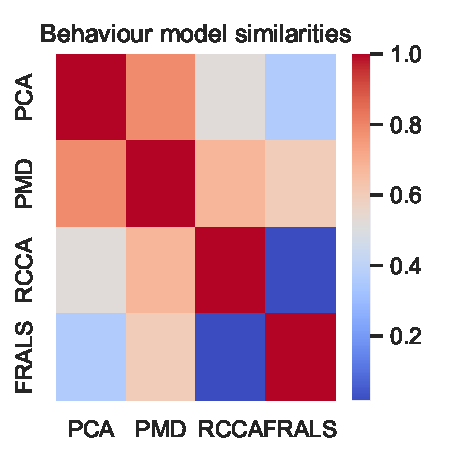
\includegraphics[width=0.49\linewidth]{figures/als/hcp/behaviour_model_similarities}
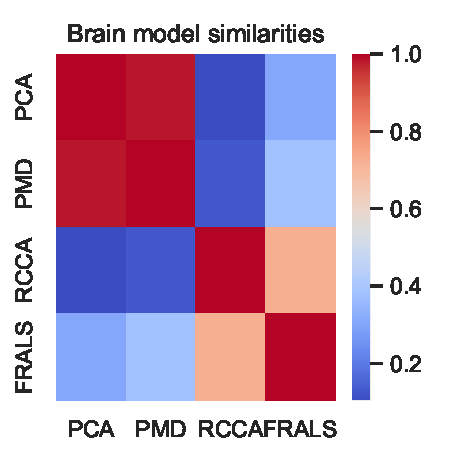
\includegraphics[width=0.49\linewidth]{figures/als/hcp/brain_model_similarities}
\caption{Left: Correlation matrix of the scores for each modality. Right: Correlation matrix of the brain loadings for each model.}
\label{fig:similarities}
\end{figure}

\subsubsection{Behaviour and Brain Loadings}
In terms of behavioral loadings, except for PCA, all models identified a latent variable that correlated positively with cognitive tests and negatively with cigarette, tobacco, or alcohol use.
Both RCCA and FRALS demonstrated stronger correlations with the Line Orientation test, which measures visuospatial abilities.

\begin{figure}[h]
\centering
\includesvg[width=\linewidth]{figures/als/hcp/all_top_and_bottom_loadings.svg}
\caption*{Top 5 positive and negative non-imaging loadings for each model}
\label{fig:behaviour}
\end{figure}

Regarding the brain loadings, our analysis shows that each model assigns different weights to various brain regions
based on their connectivity.
RCCA and FRALS assigned more weight to the parietal lobe, known for its role in visuospatial processing, than did PCA and PMD. This suggests that the parietal lobe is more relevant for the brain-behaviour correlations captured by our model.
Conversely, PMD appears to rely on principal components in the brain, potentially missing the true associations between the views.
FRALS functions as a sparse version of RCCA in this context.

\begin{figure}[h]
\centering
\includegraphics[width=0.49\linewidth]{figures/als/hcp/pca_brain_loadings}
\includegraphics[width=0.49\linewidth]{figures/als/hcp/pmd_brain_loadings}
\includegraphics[width=0.49\linewidth]{figures/als/hcp/rcca_brain_loadings}
\includegraphics[width=0.49\linewidth]{figures/als/hcp/flexals_brain_loadings}
\caption*{Map of CCA connection strength increases/decreases, with each node’s parcel map weighted by CCA edge-strength increases, summed across edges involving that node.}
\label{fig:brain}
\end{figure}

\subsection{Regularized CCA with the Alzheimer's Disease Neuroimaging Initiative (ADNI) Data}

Like the HCP data, the ADNI dataset is high-dimensional and multimodal, making it an ideal candidate for evaluating the flexibility and efficacy of our FRALS method.




\section{Discussion and Limitations}

The simulated data results emphasize the importance of aligning the model's objective with the characteristics of
the underlying signal for effective feature selection and signal capture.
Sparsity and domain-specific priors play a significant role, with IPLS+ showing the best performance among the models tested due to its positive constraint.

\subsection{Limitations}
While FRALS offers promising performance in terms of out-of-sample correlation, it does come with significant drawbacks, the most noteworthy being its computational inefficiency. Below, we outline the primary factors contributing to the slow speed of FRALS and provide some insights into the computational bottlenecks.

\subsubsection{Computational Time}\label{subsec:computational-time}
While computationally intensive, the flexibility of FRALS allows it to adapt better to the complexity inherent in real-world data sets, such as the HCP. This adaptability could be crucial when high predictive accuracy or interpretability is required.

\subsubsection{Changing Regression Targets}\label{subsec:changing-regression-targets}
Adding to the computational burden is the fact that the regression targets, i.e., the projections of the other view, are not static but change dynamically throughout the algorithm's run.
Each update to the least squares solution consequently alters the global objective, leading to a constantly shifting landscape that the algorithm needs to navigate.

\section{Conclusions}
The main idea of this chapter is to introduce FRALS, a novel approach in the realm of multiview learning that optimizes
both flexibility and performance.
Our experiments indicate that FRALS not only outperforms established methods like PCA, PMD, and RCCA in terms of out-of-sample canonical correlations but also captures novel and distinct aspects of brain-behavior associations.
This uniqueness is evident from the low or negative correlations FRALS holds with other models.

Our findings also underline the importance of the parietal lobe in understanding brain-behavior associations.
FRALS emphasizes this region more compared to traditional methods like PCA and PMD. Future work should focus on understanding the specific functions and contributions of different brain regions captured by FRALS and how they relate to various behaviors.

Given its promising initial results, the next step for FRALS would be its application to larger datasets and its adaptation for different kinds of biological and non-biological data to further evaluate its robustness and applicability.



